\documentclass[a4paper,11pt]{report} % ligne de classe
% preambule

\usepackage[utf8]{inputenc} % *nix => utf8 | latin1/latin9 => win

% pour la beauté des fontes
\usepackage[T1]{fontenc}
\usepackage{lmodern}

% parce qu'on est français
\usepackage[french]{babel}

% on veut des maths
\usepackage{amsmath}
\usepackage{amsfonts}

%schema
\usepackage{tikz}
    \usepackage[europeanresistors]{circuitikz}
    \usetikzlibrary{arrows}


\DeclareMathOperator{\sinc}{sinc}

% on veut utiliser des images
\usepackage{graphicx}
\usepackage{caption}
\usepackage{subcaption}


% définir les marge
\usepackage{geometry}
\geometry{top=3cm,left=2cm,bottom=2.5cm,right=2cm}

% en-tête et pied de page
\usepackage{fancyhdr}


% épaisseur des lignes
\renewcommand{\headrulewidth}{0.4pt}
\renewcommand{\footrulewidth}{0.4pt}

% haut
%\lhead{}
%\chead{Mon super méga document}
%\rhead{René la taupe}
% bas
%\lfoot{mon terrier}
%\cfoot{}
%\rfoot{\thepage}


% pour acitver le style "fancy"
\pagestyle{fancy}
\addto\captionsfrench{\renewcommand{\chaptername}{Partie}}
\lhead{}
\chead{}
\rhead{}
\renewcommand{\headrulewidth}{0pt}

\newcommand{\Real}{\mathrm{Re}}

%pour le trait sous les section
\usepackage{sectsty}
\sectionfont{
    \sectionrule{0pt}{0pt}{-5pt}{0.6pt}
    }

\renewcommand{\thechapter}{\arabic{chapter}}
\renewcommand{\thesection}{\arabic{section}.}
\renewcommand{\thesubsection}{\arabic{section}.\arabic{subsection}.}

\usepackage{url}


% \nom_de_la_commande[args optionnels]{arg(s) obligatoires}

% Première page
%\title{Mon super méga document}
%\author{René la Taupe}
%\date{Aujourd'hui}

\begin{document} % début du doc
% corps du doc

\begin{titlepage}

\newcommand{\HRule}{\rule{\linewidth}{0.5mm}} % Defines a new command for the horizontal lines, change thickness here

\center % Center everything on the page
 
 
%----------------------------------------------------------------------------------------
%	HEADING SECTIONS
%----------------------------------------------------------------------------------------

\textsc{\large Université du Maine \\ UFR Sciences et Techniques}\\[0.5cm] % Name of your university/college

\textsc{\Large Licence SPI 3ème année}\\[1.0cm] % Major heading such as course name
\textsc{\large Rapport de projet - Second semestre}\\[0.5cm] % Minor heading such as course title
\bigskip \bigskip

%----------------------------------------------------------------------------------------
%	TITLE SECTION
%----------------------------------------------------------------------------------------

\HRule \\[0.6cm]
{ \bfseries Étude du phénomène de dispersion}\\[0.4cm] % Title of your document
\HRule \\[1.5cm]
 
%----------------------------------------------------------------------------------------
%	AUTHOR SECTION
%----------------------------------------------------------------------------------------

\begin{minipage}{0.4\textwidth}
\begin{flushleft} \large
\emph{Étudiants :} \newline \newline
\large Thomas \textsc{\large Lechat}\\
\large Alice \textsc{\large Dinsenmeyer}\\
\end{flushleft}
\end{minipage}
~
\begin{minipage}{0.4\textwidth}
\begin{flushright} \large
\emph{Encadrant :} \newline \newline
\large Sohbi \textsc{\large Sahraoui}\\
Professeur à l'université du Maine
% Supervisor's Name
\end{flushright}
\end{minipage}\\[4cm]

% If you don't want a supervisor, uncomment the two lines below and remove the section above
%\Large \emph{Author:}\\
%John \textsc{Smith}\\[3cm] % Your name

%----------------------------------------------------------------------------------------
%	DATE SECTION
%----------------------------------------------------------------------------------------

{\large Année universitaire 2013-2014}\\[3cm] % Date, change the \today to a set date if you want to be precise

%----------------------------------------------------------------------------------------
%	LOGO SECTION
%----------------------------------------------------------------------------------------

%\includegraphics{Logo}\\[1cm] % Include a department/university logo - this will require the graphicx package
 
%----------------------------------------------------------------------------------------

\vfill % Fill the rest of the page with whitespace

\end{titlepage}

% table des matières
\tableofcontents

\newpage % saut de page

\section*{Remerciements}
Nous remercions en premier lieu Sohbi Sahraoui, notre encadrant, pour nous avoir lancé et guidé sur ce projet. Son point de vue et ses conseils nous ont été précieux.

Nous remercions également tous les professeurs de la licence qui nous ont formés pendant ces trois années, et tout particulièrement ceux qui se sont rendus disponibles pour nous durant la réalisation de ce projet.

Merci également aux divers relecteurs.
\bigskip

\section*{Résumé}
Ce projet débute par l'étude du phénomène de dispersion à travers deux exemples: la propagation d'une onde de pression guidée et celle d'une onde dans une poutre en flexion.

Dans le premier cas, la dispersion est liée à la présence des parois. Sur ces parois, l'application des conditions limites pour la pression fait apparaître des modes sur le plan perpendiculaire à l'axe de propagation de l'onde, ce qui entraîne une modification de la constante de propagation.

Dans le second cas, la prise en compte des moments de torsion lors de la mise en équation du mouvement transversal de la poutre en flexion conduit à une dérivée quatrième sur la composante spatiale du déplacement dans l'équation de propagation. La résolution de cette équation fait alors apparaître une relation de dispersion. Ce deuxième cas est confirmé expérimentalement grâce à une mesure réalisée à l'ENSIM\footnote{École nationale supérieure d’ingénierie du Mans}.

\bigskip
Dans un second temps, la dispersion liée aux réseaux réguliers est considérée avec l'étude théorique et expérimentale d'une corde en acier à laquelle sont fixées des masses à intervalles réguliers. Cette configuration périodique fait apparaître la non-propagation de certaines fréquences créant des bandes interdites ainsi que les variations de vitesse de groupe qui surviennent au voisinage de ces bandes. Cette partie est principalement réalisée en appliquant la théorie des lignes de transmission.



\chapter*{Introduction}
\addcontentsline{toc}{chapter}{Introduction}

Le phénomène de dispersion est traduit par une différence de célérité entre les différentes fréquences constituant une onde.
Il existe de nombreux cas d'ondes dispersives, telles que les ondes électromagnétiques et acoustiques guidées, certaines ondes de surface, de flexion, \emph{etc}. Tous les milieux sont plus ou moins dispersifs et ce sont les propriétés du milieu qui caractérisent la prépondérance de la dispersion. C'est, de ce fait, un phénomène très courant. \\

Ce projet de fin de licence porte sur l'étude des causes de ce phénomène dans deux types de milieux : sans et avec discontinuités.


La première partie de cette étude concerne les milieux uniformes (sans discontinuité), avec en premier lieu, une analyse des modes dans un guide d'onde rectangulaire et en second lieu une modélisation des ondes mécaniques dans une poutre en flexion. Pour ces deux cas, les relations théoriques liées à la dispersion ont été établies ; en complément du travail réalisé sur la poutre, une vérification expérimentale a été menée.
 
 
La seconde partie est consacrée à un réseau à pas régulier constitué de masses ponctuelles fixées sur une corde vibrante. Travail théorique et simulation numérique sont confrontés à une analyse expérimentale temps-fréquences réalisée à l'aide de la transformée de Fourier à court terme (spectrogramme).

\setcounter{section}{0}

\chapter{Approche de la dispersion dans un milieu uniforme}
Dans cette section, deux exemples de dispersion en milieu uniforme sont traités. Les deux systèmes étudiés sont le guide d'onde en 2 dimensions et la poutre encastrée-libre en flexion. 

L'objectif est principalement d'introduire les notions de vitesse de phase et de groupe, ainsi que les méthodes de visualisation de la dispersion.	


\section{Dispersion dans un guide d'onde rectangulaire}

L'objectif étant de se familiariser avec le phénomène de dispersion, une étude succincte de la propagation d'une onde dans un guide est réalisée.

Afin de simplifier le problème, le guide considéré est en 2 dimensions, de hauteur L et les pertes ne sont pas prises en compte.

\subsection{Mise en équation du problème}

La propagation de l'onde de pression $p$ dans le guide est donnée par l'équation de propagation : 
\begin{equation*}
\nabla^2p - \frac{1}{c^2}\frac{\partial{^2p}}{\partial{t}^2} = 0
\end{equation*}
Avec $c$ la célérité des ondes planes dans le guide.

\subsubsection{Expression de la pression en régime harmonique}

En considérant tout d'abord une seule fréquence, $p(\omega,t) = P(x,y)e^{j\omega t}$, on a l'équation d'Helmholtz : 
\begin{equation}\label{helm}
\nabla^2p + k^2p = O \qquad \text{ avec } k = \frac{\omega}{c}
\end{equation}


On utilise la méthode des séparation des variables: on pose $P(x,y) = X(x)Y(y)$, on peut alors transformer l'équation d'onde avec les notations suivantes:
\begin{equation*}
\frac{\partial{^2X}}{\partial{x^2}} = X'' \qquad \text{et} \qquad \frac{\partial{^2Y}}{\partial{y^2}} = Y'' 
\end{equation*}

L'équation d'Helmholtz~\ref{helm} devient alors :
\begin{equation*}
\frac{X''}{X} +\frac{Y''}{Y} + k^2 = 0
\end{equation*}

Cette relation permet d'obtenir l'amplitude de la pression au point de coordonnées $(x,y)$ (en ne considérant que l'onde se propageant suivant les x croissants) : 

\begin{eqnarray*}
	 \frac{Y''}{Y} = -k_y^2 \qquad & \Rightarrow & \qquad Y = A\cos{k_yy}+B\sin{k_yy} \\~ \\
	 \frac{X''}{X} = k_x^2 = k^{2} - k_y^2 \qquad & \Rightarrow & \qquad X = Ce^{-k_xx}
\end{eqnarray*}

D'où, finalement : $p(x,y,t) = X(x)Y(y)e^{jwt} =   [A\cos{k_yy}+B\sin{k_yy}]Ce^{-k_xx} e^{jwt}$.

\subsubsection{Conditions limites}
En supposant que les parois sont infiniment rigides, on à la condition limite suivante suivant $(O_y)$: 
\begin{equation*}
\left.\frac{\partial{p}}{\partial{y}}\right|_{\begin{smallmatrix}y=0 \\ y=L\end{smallmatrix}} = 0
\end{equation*}
On a donc : \begin{equation*}
				\begin{cases}
					k_yB\cos(k_yy) = 0 \qquad \Rightarrow \qquad B = 0 \\
					-k_yA\sin(k_yL) = 0 \quad \Rightarrow \qquad k_{yn} = \frac{n\pi}{L}
				\end{cases}
		\end{equation*}


Finalement,	\begin{equation*}
				P(x,y) = \sum_n A_n \cos\left(\frac{n\pi}{L}y\right)e^{-k_{xn}x}
			\end{equation*}
avec \begin{equation*}
			k_{xn} =\sqrt{k^2-k_{yn}^2}= \sqrt{k^2-\left(\frac{n\pi}{L}\right)^2}
		\end{equation*}

On distingue alors deux cas : 

\begin{itemize}
\item celui où $k_{xn}$ est imaginaire pur, c'est-à-dire en dessous de la première fréquence de coupure du guide, quand $k<\frac{n\pi}{L}$. L'onde est alors évanescente.
\item celui où $k_{xn}$ est purement réel, c'est-à-dire quand $k>\frac{n\pi}{L}$. L'onde est alors propagative.
\end{itemize}

\subsection{Vitesse de phase}	
La vitesse de phase, notée $c_{ph}$, est définie ainsi pour chaque mode n : 
\begin{equation*}
c_{ph_n} = \frac{\omega}{k_{xn}} = \frac{c}{\sqrt{1-\left(\frac{n\pi}{kL}\right)^2}}
\end{equation*}

Cette vitesse de phase dépend donc de la fréquence et du mode. Le guide est donc un milieu dispersif au-delà du premier mode correspondant à $n=0$.

La figure~\ref{graph_c_phase} montre l'évolution de cette vitesse de phase en fonction de la fréquence et des modes dans un guide de 30 cm de largeur et dont la vitesse du mode plan est de 340 m/s. 
Ces courbes font apparaître le nombre de modes propagatifs pour chaque fréquence. Par exemple, à 3000 Hz, seuls les cinq premiers modes sont propagatifs (modes de 0 à 4).

\begin{figure}[h!]
\centering 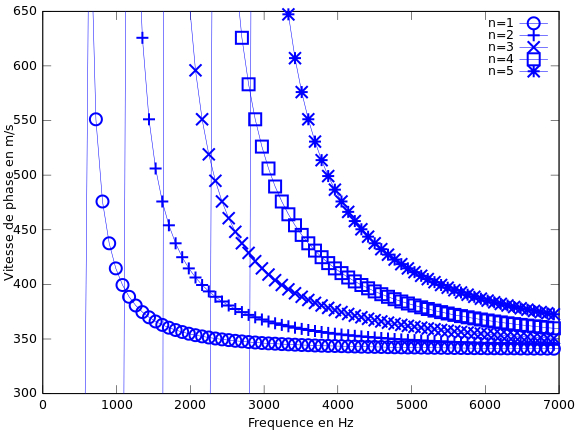
\includegraphics[scale = 0.6]{./figures/c_phase.jpg}
\caption{Évolution de la vitesse de phase en fonction de la fréquence, dans un guide rectangulaire, pour les 5 premiers modes (L = 30 cm, c = 340 m/s).} \label{graph_c_phase}
\end{figure}

\subsection{Vitesse de groupe}

La vitesse de groupe correspond à la propagation de l'énergie ou à la vitesse de l'enveloppe du paquet d'ondes. Elle est tracée en figure~\ref{graph_c_groupe} et est définie par l'équation : 
\begin{equation}
c_{gn} = \frac{\mathrm{d}\omega}{\mathrm{d}k_{xn}} = c\sqrt{1-\left(\frac{n\pi}{kL}\right)^{2}}
\end{equation}

\begin{figure}[h!]
\centering 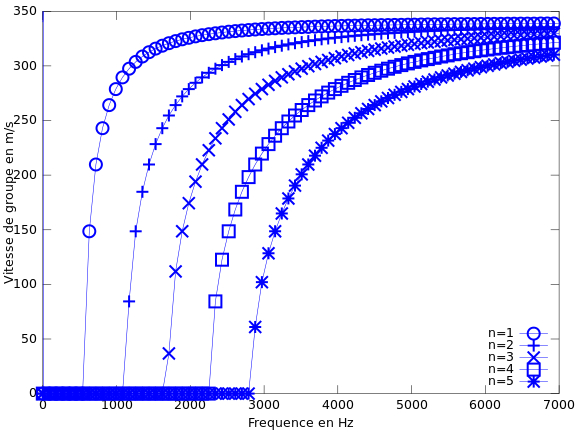
\includegraphics[scale = 0.6]{./figures/c_groupe.jpg}
\caption{Évolution de la vitesse de groupe en fonction de la fréquence, dans un guide rectangulaire, pour les 5 premiers modes (L = 30 cm, c = 340 m/s).} \label{graph_c_groupe}
\end{figure}


\bigskip
De manière à rendre visuels le concept de vitesse de groupe, une vidéo basée sur l'effet de Moiré est réalisée. Cette vidéo est une simulation de deux réseaux de lignes se déplaçant à des vitesses différentes.
Dans notre cas, chaque réseau représente les maximums de pression d'une onde de pulsation $\omega_i = 2\pi f_i$. Les deux réseaux ne se déplacent pas à la même vitesse en raison de la dispersion.

Cela équivaut à sommer les deux signaux suivants : 
\begin{eqnarray}
	\begin{cases}
		p_1 = A\cos(\omega_1t-k_1x) \\
		p_2 = A\cos(\omega_2t-k_2x)
	\end{cases} 
	\qquad \Rightarrow \qquad p_1+p_2 =2A\cos\left(\Delta \omega t-\Delta kx\right)\cos\left(\omega_0 t-k_0x\right)
\end{eqnarray}
avec
\begin{equation*}
\Delta \omega = \frac{\omega_1-\omega_2}{2} \qquad \text{,~} \qquad \Delta k = \frac{k_1-k_2}{2} \qquad \text{,~} \qquad  \omega_0 = \frac{\omega_1+\omega_2}{2} \qquad \text{ et } \qquad  k_0 = \frac{k_1+k_2}{2}
\end{equation*}

L'effet de battement visible sur la vidéo permet de visualiser la vitesse de groupe : $c_g = \frac{\Delta \omega}{\Delta k}$.

La vitesse de phase n'est pas visible car seuls les maximums de pression sont représentés.

Cette video est disponible à l'adresse suivante :\\
\url{http://perso.univ-lemans.fr/~s112653/projet_dispersion/moire_dispersion.avi}


\bigskip \bigskip

Finalement, le guide est un milieu dispersif car la vitesse de phase et la vitesse de groupe sont une fonction de la pulsation.
Dans le cas où le milieu n'est pas dispersif, le paquet d'onde composé des différentes ondes monochromatiques ne se déforme pas. On a alors : $c=c_p=c_g$.


\vspace{2cm}




\section{Vibration d'une poutre en flexion}
On cherche ici à mettre en évidence la différence de célérité entre 2 ondes de fréquences proches se propageant dans une poutre encastrée-libre ainsi que les fréquences de résonances de celle-ci.

On s'intéresse donc au petit élément d'une poutre de dimensions constantes représenté sur la figure \ref{poutre_graphic1} sur laquelle $M(x)$ est le moment de torsion en $x$ et $T(x)$ est l'ensemble des forces internes à la poutre en $x$.

\begin{figure}[!h]
\centering{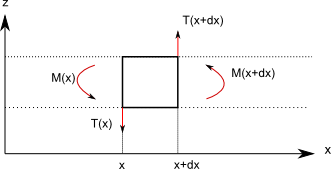
\includegraphics[scale=1.1]{./figures/segment_poutre.png}}
\caption{\label{poutre_graphic1} Forces s’exerçant sur un élément de longueur $dx$ d'une poutre en flexion}
\end{figure}

La poutre est de section uniforme et l'on suppose un encastrement parfait. De plus, au vu des dimensions de la poutre et du type d'excitation, seul le mouvement de flexion est considéré.

\subsection{Détermination de l'équation de propagation dans la poutre}
On fait tout d'abord une approximation sur $T(x+dx)$ et $M(x+dx)$ en considérant que $dx$ est extrêmement faible, d'où : 

\begin{eqnarray*}
\begin{cases} M(x+dx) = M(x) + \frac{\partial M(x)}{\partial x} dx  \\ T(x+dx) = T(x) + \frac{\partial T(x)}{\partial x} dx  \end{cases}
\end{eqnarray*}

On applique ensuite le principe fondamental de la dynamique à l'élément de poutre considéré. Si on appelle $W$ le déplacement transversal de la poutre, on obtient :

\begin{eqnarray*}
&& \sum F_{ext} = \frac{\partial ^2 W}{\partial t^2} dm \\
&  \Leftrightarrow & T(x+dx) - T(x) = \frac{\partial ^2 W}{\partial t^2} \rho S dx\\
&  \Leftrightarrow & \frac{T(x+dx) - T(x)}{dx} = \rho S \frac{\partial ^2 W}{\partial t^2} \\
& \Leftrightarrow & \frac{\partial T(x)}{\partial x} = \rho S \frac{\partial ^2 W}{\partial t^2}
\end{eqnarray*}

Grâce au théorème des moments, on sait que :
\begin{eqnarray*}
M(x) & = & M(x+dx) + T(x) dx \\
 & = & M(x) + \frac{\partial M}{\partial x} dx + T(x) dx \\
 &  \Leftrightarrow & -\frac{\partial M(x)}{\partial x} = T(x) \\
 &  \Leftrightarrow & - \frac{\partial ^2 M(x)}{\partial x^2} = \frac{\partial T(x)}{\partial x}
\end{eqnarray*}

En réinjectant cette dernière formule dans le principe fondamental de la dynamique appliqué à l'élément de poutre, on obtient : 
\begin{eqnarray*}
\frac{\partial T(x)}{\partial x} = \rho S \frac{\partial ^2 W}{\partial t^2} = -\frac{\partial ^2 M(x)}{\partial x^2}
\end{eqnarray*}

On doit donc chercher une expression du moment en fonction de la position de la poutre :

\begin{eqnarray*}
dM(x) = z dF \qquad \Rightarrow \qquad M(x) = \int_S z dF 
\end{eqnarray*}

Or:
\begin{eqnarray*}
dF = -E z \frac{\partial ^2 W}{\partial x^2} dS
\end{eqnarray*}

On peut donc calculer $M(x)$ :

\begin{eqnarray*}
M(x) = - \int_S E z^2 \frac{\partial ^2 W}{\partial x^2} dS = E I \frac{\partial ^2 W}{\partial x^2}
\end{eqnarray*}
Où $I$ est le moment quadratique de la poutre.

En remplaçant $M(x)$ dans le principe fondamental de la dynamique, on obtient finalement :
\begin{equation}\label{eq1}
\rho S \frac{\partial ^2 W}{\partial t^2} = -E I \frac{\partial ^4 W}{\partial x^4}
\end{equation}


Cette équation n'est pas une équation d'onde classique du fait du terme de dérivation quatrième, cependant ses solutions sont des ondes, et on peut d'ores et déjà supposer que c'est de ce terme que vient la dispersion. 

\subsection{Résolution par la méthode de séparation des variables}
On cherche ici à trouver la solution générale de l'équation \ref{eq1}.

On pose : $W(x,t) = f(x) g(t)$. On peut donc écrire l'équation \ref{eq1} de la manière suivante :
\begin{eqnarray*}
\frac{1}{g(t)} \rho S \frac{\partial ^2 g(t)}{t^2} = -\frac{EI}{f(x)} \frac{\partial ^4 f(x)}{\partial x^4} = \alpha \\
\Rightarrow \begin{cases}
{\partial ^2 g(t)}{\partial t^2} = \alpha g(t) \\~\\ \frac{\partial ^4 f(x)}{\partial x^4} = - \frac{\alpha \rho S}{EI} f(x)\end{cases}
\end{eqnarray*}

On pose $\alpha = -\omega^2$ car on sait que les solutions temporelles n'auront pas de sens physique dans le cas où $\alpha$ est négatif.


On obtient immédiatement pour les solutions temporelles :
\begin{eqnarray*}
g(t) = A \cos(\omega t) + B \sin(\omega t) \\
g'(t) = -A\omega \sin(\omega t) + B\omega \cos(\omega t)
\end{eqnarray*}

Pour la dépendance spatiale, on a l'équation caractéristique suivante :
\begin{eqnarray*}
r^4 - \frac{ \rho S \omega^2}{EI} = 0
\qquad \Rightarrow \qquad\begin{cases} r = \pm \beta  \\ r = \pm i\beta \end{cases} \text{ avec } \beta = \sqrt[4]{\frac{\rho S \omega^2}{EI}}
\end{eqnarray*}

On obtient donc les solutions spatiales suivantes:
\begin{eqnarray*}
f(x) & = & c e^{i\beta x} + d e^{-j\beta x} + f e^{\beta x} + g e^{-\beta x} \\
\Leftrightarrow f(x) & = & C \cos(\beta x) + D \sin(\beta x) + F \cosh(\beta x) + G \sinh(\beta x)
\end{eqnarray*}

On peut, de plus, exprimer la relation de dispersion du système car on a: $ \frac{\omega}{\beta}=c$. D’où la relation:
\begin{equation}
\beta = \sqrt[4]{\frac{\rho S \omega^2}{EI}} \qquad \Leftrightarrow \qquad \sqrt[4]{\frac{EI}{\rho S}} \beta = \sqrt{\omega} \qquad \Leftrightarrow \qquad c_{phase} = \frac{\omega}{\beta} = \sqrt{\omega} \sqrt[4]{\frac{EI}{\rho S}}
\end{equation}

Cette relation de dispersion est représentée figure ~\ref{poutre_graphic2}.

\begin{figure}[h!]
\centering 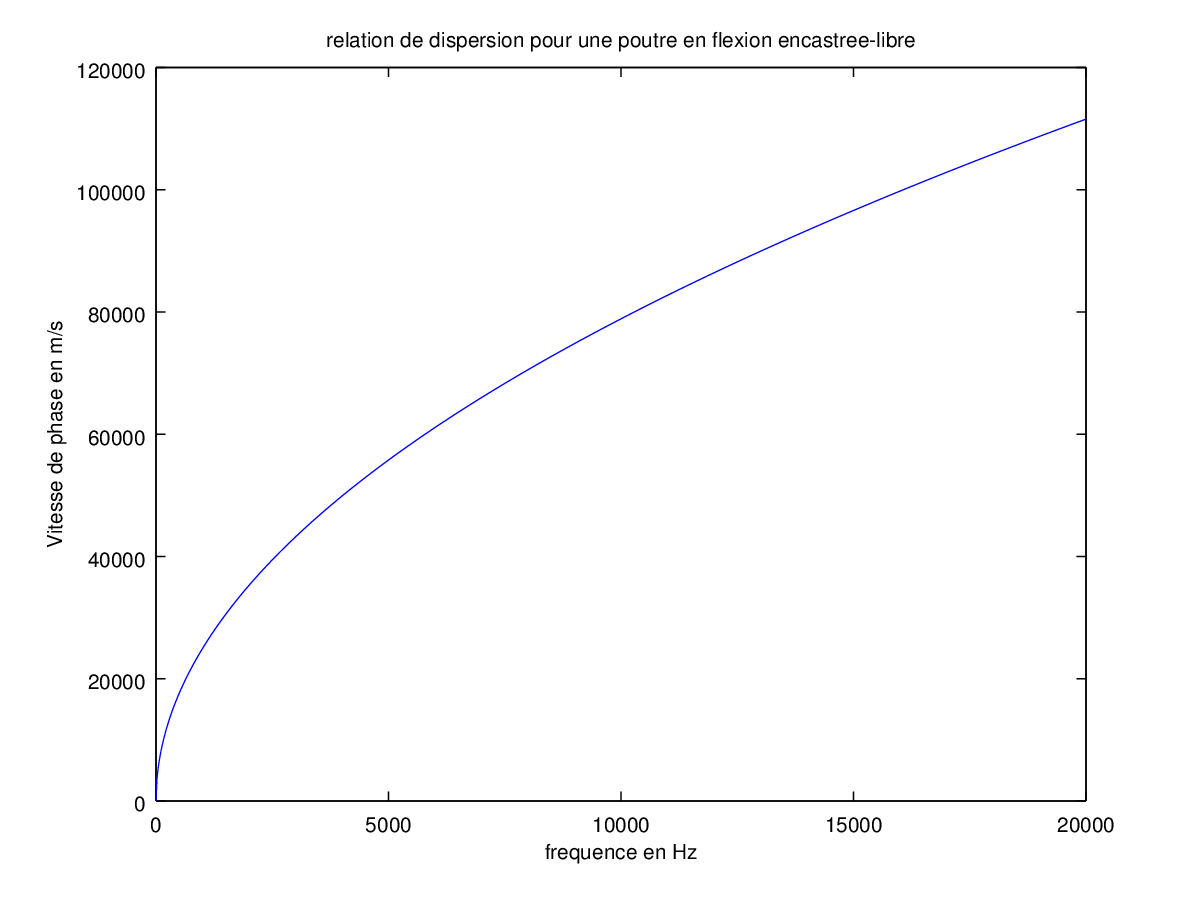
\includegraphics[scale = 0.6]{./figures/poutre_dispersion.png}
\caption{Relation de dispersion d'une poutre en acier de 3~m de longueur, 2~cm d'épaisseur et 10~cm de largeur.   } \label{poutre_graphic2}
\end{figure}

On constate que la courbe n'est pas une droite linéaire, les poutres en flexion sont donc dispersives et ce quelque soit les conditions limites utilisées. Cependant la dispersion doit être visible sur l'écart entre les fréquences de résonance pour des conditions limites fixées, cette hypothèse va donc être vérifiée dans la suite.

\subsection{Application des conditions limites}

En $x=0$ ce trouve l'encastrement, on a donc:
\begin{eqnarray*}
\begin{cases} W(0,t) = 0 \\ \frac{\partial W(0,t)}{\partial x} = 0 \end{cases}
\end{eqnarray*}

En $x=L$, la poutre est libre, le moment fléchissant ainsi que l'effort tranchant est donc nul. On a donc:

\begin{eqnarray*}
\begin{cases}  EI \frac{\partial ^2 W(L,t)}{\partial ^2 x} = 0 \\ EI \frac{\partial ^3 W(L,t)}{\partial x^3} = 0 \end{cases}
\end{eqnarray*}

On a de plus:
\begin{eqnarray*}
f(x) & = & C \cos(\beta x) + D \sin(\beta x) + F \cosh(\beta x) + G \sinh(\beta x) \\
f'(x) & = & -C \beta \sin(\beta x) + D \beta \cos(\beta x) + F \beta \sinh(\beta x) + G \beta \cosh(\beta x) \\
f''(x) & = & -C \beta ^2 \cos(\beta x) - D \beta ^2 \sin(\beta x) + F \beta ^2 \cosh(\beta x) + G \beta ^2 \sinh(\beta x) \\
f'''(x) & = & C \beta ^3 \sin(\beta x) - D \beta ^3 \cos(\beta x) + F \beta ^3 \sinh(\beta x) + G \beta ^3 \cosh(\beta x) \\
\end{eqnarray*}

On a donc pour l'encastrement:
\begin{eqnarray*}
\begin{cases} 
C + F = 0  \\ 
D + G = 0  
\end{cases}
\Leftrightarrow  \qquad
\begin{cases}
C = -F \\
D = -G 
\end{cases}
\end{eqnarray*}

Et pour la partie libre, en prenant en compte la condition d'encastrement:
\begin{eqnarray*}
\begin{cases} 
C \beta ^2 [\cos(\beta L) + \cosh(\beta L)]+ D \beta ^2 [\sin(\beta L) + \sinh(\beta L)] = 0 \\
C \beta ^2 [\sinh(\beta L) -\sin(\beta L)] + D \beta ^2 [\cos( \beta L) + \cosh(\beta L)] = 0
\end{cases} \\
\Leftrightarrow \begin{cases} 
C [\cos(\beta L) + \cosh(\beta L)]+ D [\sin(\beta L) + \sinh(\beta L)] = 0    ~~(1)\\
C [\sinh(\beta L) -\sin(\beta L)] + D [\cos( \beta L) + \cosh(\beta L)] = 0  ~~ (2)
\end{cases} \\
\end{eqnarray*}

On peut ainsi aboutir à une équation transcendantale:
\begin{eqnarray*}
(2) & \Rightarrow & C = \frac{D[\cos(\beta L) + \cosh(\beta L)]}{\sin(\beta L) - \sinh(\beta L)} \\
(2) \rightarrow (1) & \Rightarrow & D[\cos(\beta L) + \cosh(\beta L)]^2 + D [\sin^2(\beta L) + -\sinh^2(\beta L)] = 0 \\
& \Leftrightarrow & D[\cos^2(\beta L) + \cosh^2(\beta L) + 2 \cos(\beta L) \cosh(\beta L)] + D[\sin^2(\beta L) - \sinh^2(\beta L)] = 0 \\
& \Leftrightarrow & \sin^2(\beta L) + \cos^2(\beta L) + \cos^2(\beta L) - \sinh^2(\beta L) + 2\cos(\beta L) \cosh(\beta L) = 0 \\
& \Leftrightarrow & 2\cos(\beta L)\cosh(\beta L) = -2 \\
& \Leftrightarrow & \cos(\beta L) \cosh(\beta L) = -1
\end{eqnarray*}

Cette équation ne peut pas être résolue analytiquement. Cependant un calcul numérique permet d'avoir des solutions approchées.
Si on pose $\beta L = R_n$, on a alors: 
\begin{equation}
f_n = \frac{R_n^2}{L^2} \sqrt{\frac{EI}{\rho S}}
\label{form1}
\end{equation}

On peut donc en déduire les premières fréquences propres grâce aux valeurs approchées de $R_n^2$. Celles-ci sont disponibles tableau \ref{tab1}.


\bigskip
\begin{minipage}[c]{\textwidth}
\centering
\begin{tabular}{c|c|c }
Numéro $n$ du mode  & Valeur de $R_n$ & Valeur de $R_n^2$\\\hline
0 & 1.8751 &3.5160\\
1 &  4.6941 &22.035\\
2 & 7.8547 &61.696\\ 
$\ge$ 3 & $\frac{\pi}{2}(2n-1)$ & $\frac{\pi}{2}(2n-1)^2$
\end{tabular}
\captionof{table}{ \label{tab1} Valeurs approchées de $R_n$ permettant de calculer les fréquences propres pour une poutre encastrée-libre.}
\end{minipage}

\bigskip
On constate que les fréquences propres ne sont pas multiples de la fondamentale, ce dernier point peut donc être utilisé pour déterminer si oui ou non un système est dispersif.


\subsection{Vérification expérimentale de la dispersion}
La poutre étudiée a pour longueur $L = 63.5~ cm$, est constituée d'aluminium de module d'Young $E = 70~GPa$ et de masse volumique $\rho = 2700~kg/m^3$. Sa largeur est de $b = 30~mm$ et sa hauteur de $h=5~mm$.

Le dispositif est constitué d'un pot vibrant excitant une poutre encastrée-libre sur laquelle est fixée un accéléromètre (voir figure \ref{schema}). 

\begin{figure}[!h]
\centering{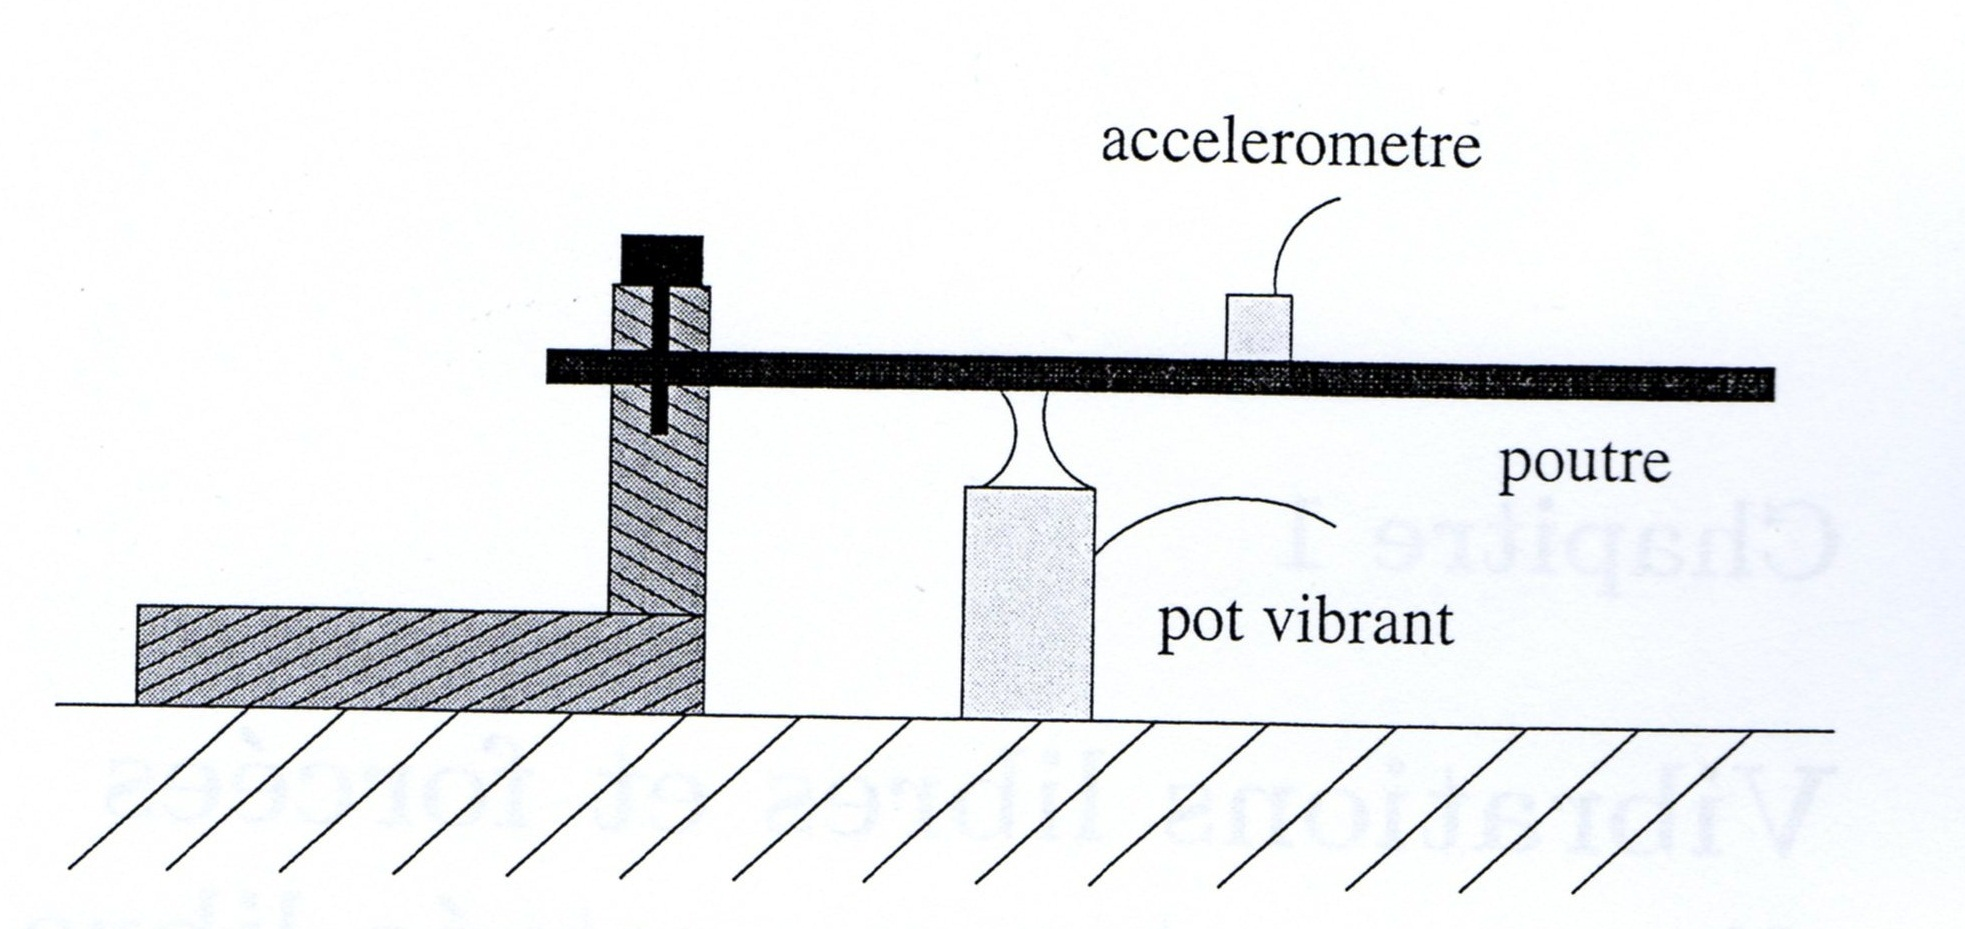
\includegraphics[scale=0.7]{./figures/schema_poutre2.jpg}}
\caption{\label{schema} Schéma du dispositif (extrait des sujets de TP d'analyse modale).}
\end{figure}

On réalise une réponse en fréquence à partir du signal du capteur afin de visualiser les fréquences de résonance de la poutre. Le pot vibrant excite le système avec un chirp linéaire allant de O à $1000Hz$.

Les fréquences propres obtenues ainsi que les valeurs théoriques de celles-ci calculées \emph{via} la formule~\ref{form1} sont présentées dans le tableau~\ref{tab2}.

\bigskip
\begin{minipage}[c]{\textwidth}
\centering
\begin{tabular}{c|c|c|c }
Numéro du mode & Fréquence mesurée  & $R_n$ du mode & Valeur théorique \\\hline
1 & 9.7 Hz & 1.875 & 10.20 Hz\\
2 & 60.5 Hz & 4.694 & 63.92 Hz\\
3 & 170 Hz & 7.855 & 179.00 Hz\\
4 & 320 Hz & 10.996 & 350.00 Hz\\
5 & 707 Hz & 14.137 & 579.7 Hz \\
6 & - & 17.279 & 866.1 Hz
\end{tabular}
\captionof{table}{ \label{tab2} Fréquences propres théoriques et relevées expérimentalement pour une poutre encastrée-libres.}
\end{minipage}

\bigskip
On constate que les fréquences mesurées et expérimentales sont à peu près les mêmes pour les basses fréquences mais les erreurs augmentent beaucoup en hautes fréquences.  Cela peut être dû à l'approximation faite sur les $R_n$ en hautes fréquences ou même l'intrusivité du pot vibrant.

\bigskip \bigskip
Cependant la dispersion d'une onde ne se rapporte pas seulement à un changement de la vitesse de l'onde en fonction de la fréquence. D'autres phénomènes liés à la dispersion entrent en jeu, phénomènes qui sont étudiés dans le chapitre suivant.





\chapter{Étude de la dispersion dans un réseau à pas régulier}
Dans cette seconde partie nous allons étudier un système constitué d'une corde tendue à laquelle sont fixées $N$ masses de poids négligeables devant la tension de la corde.

\section{Modélisation d'une portion de la corde}

On s'intéresse tout d'abord à un élément de corde seule. Celui-ci est représenté sur le schéma \ref{schema_corde}, où $\mu$ est la masse linéique de la corde et $T$ les tensions dans la corde.\\

\begin{figure}[!h]
\centering{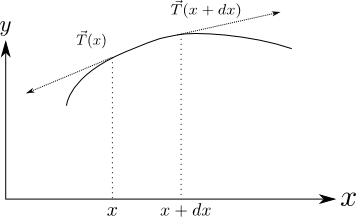
\includegraphics[scale=0.6]{./figures/schema_corde.png}}
\caption{\label{schema_corde} Schéma d'une corde vibrante sans masses ponctuelles}
\end{figure}



\subsection{Mise en équation de la corde sans masse}
En appliquant le principe fondamental de la dynamique à cet élément, on obtient l'équation suivante:
\begin{eqnarray*}
\mu dx \vec{a} (x) = \vec{T}(x) + \vec{T} (x+dx) \\
\end{eqnarray*}
Où $\mu$ est la masse linéique de la corde et $\vec{T}$ la tension dans la corde.

\indent En projetant sur l'axe (Ox), on a : 
\begin{eqnarray*}
T_x (x)= T_x (x+dx)  \qquad \Rightarrow \qquad T_x = T_0
\end{eqnarray*} 

Et suivant l'axe (Oy), on a : 
\begin{eqnarray*}
\mu dx \frac{\partial ^2 y}{\partial t^2} = -T_y (x) + T_y (x+dx)\qquad \Rightarrow \qquad \mu \frac{\partial v_y}{\partial t} = \frac{\partial T_y}{\partial t}
\end{eqnarray*}
Avec $y$ la position de la corde et $v_y$ ça vitesse suivant l'axe $(O_y$.


~\\ \indent
Or, par des considérations géométriques, on sait que:
\begin{eqnarray*}
&& \frac{T_y}{T_x} = \frac{dy}{dx} \\
& \Rightarrow & v_y = \frac{T_y}{T_0} \\
& \Rightarrow & \frac{\partial v_y}{\partial x} = \frac{1}{T_0} \frac{\partial T_y}{\partial t}
\end{eqnarray*}

On obtient donc finalement les deux équations suivantes:
\begin{equation}
\frac{\partial T_y}{\partial x} = \mu \frac{\partial v_y}{\partial t} \qquad \text{et} \qquad
\frac{\partial v_y}{\partial x} = \frac{1}{T_0} \frac{\partial T_y}{\partial t}
\label{eq2}
\end{equation}

En fusionnant ces deux équations, on tombe sur une équation d'onde sur la tension ou bien la vitesse de déplacement de la corde.

\subsection{Mise sous forme matricielle}
On s'intéresse ici à l'équation d'onde suivante tirée des équations \ref{eq2}.
\begin{equation}
\frac{\partial ^2 T}{\partial x^2} -\frac{1}{c^{2}} \frac{\partial ^2 T}{\partial t^2}= 0 \qquad \text{avec} \qquad c = \sqrt	 \frac{T_0}{\mu}
\end{equation}

On se place en régime harmonique et on note $\Gamma = jk = j\omega\sqrt{\frac{\mu}{T_0}}$ la constante de propagation du système. On sait que les solutions sont donc de la forme $T(x) = A e^{-\Gamma x} + B e^{\Gamma x}$. En réutilisant les équations \ref{eq2} et en posant $v_y=v$ par souci de simplicité, on a donc finalement:
\begin{eqnarray*}
\begin{cases}
T(x_1)  =  A e^{-\Gamma x_1} + B e^{\Gamma x_1} \\
v(x_1)  =  -\frac{1}{j\omega\mu} [ -\Gamma A e^{-\Gamma x_1} + \Gamma e^{\Gamma x_1}]\\
T(x_2)  =  A e^{-\Gamma x_2} + B e^{\Gamma x_2} \\
v(x_2)  =  -\frac{1}{j\omega\mu} [ -\Gamma A e^{-\Gamma x_2} + \Gamma e^{\Gamma x_2}]
\end{cases}
\end{eqnarray*}

où $x_1$ et $x_2$ correspondent à l'entrée et la sortie d'un élément de corde de longueur $L$. 
On pose $x_1 - x_2 = L$. Tous calculs faits, on trouve finalement:
\begin{eqnarray*}
\begin{pmatrix} T(x_1) \\ v(x_1) \end{pmatrix} = \begin{pmatrix} \cosh(\Gamma L) & \frac{j\omega\mu}{\Gamma} \sinh(\Gamma L) \\  \frac{\Gamma}{j\omega\mu}\sinh(\Gamma L) & \cosh(\Gamma L) \end{pmatrix} \begin{pmatrix} T(x_2) \\ v(x_2) \end{pmatrix}
\end{eqnarray*}

Cette matrice peut, dans notre cas, être simplifiée, car $\Gamma = jk$ :
\begin{eqnarray*}
\begin{pmatrix} T(x_1) \\ v(x_1) \end{pmatrix} = \begin{pmatrix} \cos(k L) & j \sqrt{\mu T_0} \sin(k L) \\ \frac{1}{\sqrt{\mu T_0}} \sin(k L) & \cos(k L) \end{pmatrix} \begin{pmatrix} T(x_2)\\ v(x_2) \end{pmatrix}
\end{eqnarray*}
On doit ensuite ajouter à ce modèle une masse.

\subsection{Ajout d'une masse ponctuelle}
On ajoute la masse représentée sur la figure \ref{masse_graphic}.

\begin{figure}[h!]
\centering 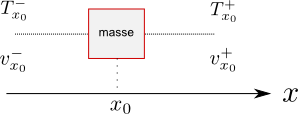
\includegraphics[scale = 1]{./figures/masse_graphic.png}
\caption{Schéma d'un élément du réseau composé d'une masse et 2 morceaux de corde \label{masse_graphic}}
\end{figure}

Les conditions limites suivantes peuvent donc être établies :
\begin{eqnarray*}
T_{x_0}^{-} = T_{x_0^{+}} + \alpha \\
v_{x_0}^{-} = v_{x_0^{+}} = v
\end{eqnarray*}

Le principe fondamental de la dynamique est ensuite appliqué à la masse, son poids est négligé du fait que celui-ci est faible au regard de la tension de la corde.
\begin{eqnarray*}
M \frac{\partial v}{\partial t} = T_{x_0^{-}} - T_{x_0^{+}} \\
\Rightarrow T_{x_0^{-}} = j \omega M v + T_{x_0^{+}}
\end{eqnarray*} 

La matrice de transfert de cette masse est ensuite déduite de cette dernière équation ainsi que de la deuxième condition limite :
\begin{equation}
\begin{pmatrix} T_{x_0^{-}} \\ v_{x_0^{-}} \end{pmatrix} = \begin{pmatrix} 1 & j \omega M \\ 0 & 1 \end{pmatrix}\begin{pmatrix} T_{x_0^{+}} \\ v_{x_0^{+}} \end{pmatrix}
\end{equation}

Cette matrice n'est donc valable que dans le cas de masses de poids relativement faible.

\section{Modélisation d'un réseau infini}
On s'intéresse ici à une cellule composée de 2 portions de corde, chacune de longueur L, avec une masse au milieu. Celle-ci peut donc être modélisé par le système matriciel suivant :
\begin{eqnarray*}
\begin{pmatrix} T_{x_0}^{-} \\ v_{x_0}^{-} \end{pmatrix} & = & \begin{pmatrix} \cos(k L) & j \sqrt{\mu T_0} \sin(k L) \\ \frac{1}{\sqrt{\mu T_0}} \sin(k L) & \cos(k L) \end{pmatrix} \begin{pmatrix} 1 & j \omega M \\ 0 & 1 \end{pmatrix}  \begin{pmatrix} \cos(k L) & j \sqrt{\mu T_0} \sin(k L) \\ \frac{1}{\sqrt{\mu T_0}} \sin(k L) & \cos(k L) \end{pmatrix} \begin{pmatrix} T_{x_0}^{+} \\ v_{x_0}^{+} \end{pmatrix} \\
& = & \begin{pmatrix} T_{11} & T_{12}\\ T_{21} & T_{22} \end{pmatrix} \begin{pmatrix} T_{x_0}^{+} \\ v_{x_0}^{+} \end{pmatrix}
\end{eqnarray*}

Avec :
\begin{eqnarray*}
T_{11} &  = & \cos^{2}(k L) + \frac{j}{Zc} \sin(k L)[j \omega M \cos(k L) + jZc \sin(k L)] \\
T_{12} &  = & j Zc \cos(k L)\sin(k L) + \cos(k L)[j \omega M \cos(k L) + j Zc \sin(k L] \\
T_{21} &  = & \frac{j}{Zc} \cos(k L) \sin(k L) + \frac{j}{Zc} \sin(k L)[\cos(k L) - \frac{\omega M}{Zc} \sin(k L)] \\
T_{22}  &=&  -\sin^{2}(k L) + \cos(k L)[\cos(k L) - \frac{\omega M}{Zc} \sin(k L)] \\ 
& = &  \cos(kd) - \frac{\omega M}{2 Zc}\sin(kd)
\end{eqnarray*}
avec $d = 2L$.

Il est notable que $T_{11} = T_{22}$ ce qui est normal pour un système symétrique est réciproque [DAL].


$T_{22}$ donne directement l'équation de dispersion pour un réseau composé d'un nombre infini de cellules : 
\begin{equation}\label{relation_dispersion}
	\cos(\Gamma d) = T_{22} = \cos(kd) - \frac{\omega M}{2 Zc}\sin(kd)
\end{equation}
avec $\Gamma$ la constante de propagation de la cellule fil-masse-fil.

Cette équation permet de caractériser la réponse en fréquence du système.
Pour que $\Gamma $ soit réel, il faut que $ -1 < T_{22} <1$. Si ce n'est pas le cas, l'onde sera évanescente et donc ne se propagera pas.
On trace donc $\cos(\Gamma d) = f(kd)$ sur la figure \ref{cordel_graphic1}.

\begin{figure}[!h]
\centering{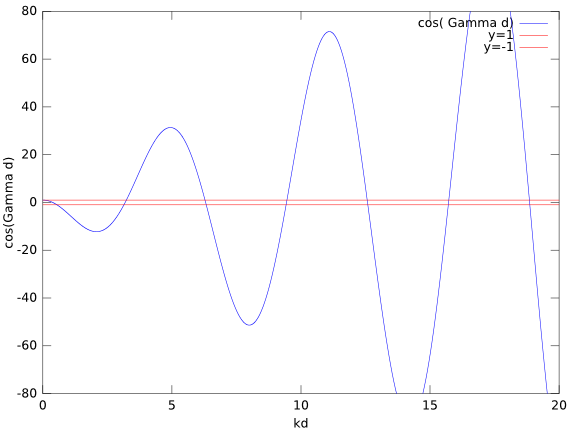
\includegraphics[width=400pt,height = 200pt]{./figures/ex_disp_cordeleste.png}}
\caption{\label{cordel_graphic1} Représentation de l'équation de dispersion pour une corde lestée}
\end{figure}

Les valeurs de $\mu$, $T_0$ et $L$ sont les mêmes que celles utilisées dans la partie expérimentales.
On constate que des bandes interdites sont présentes et que, dans le cadre de cette simulation, très peu de fréquences permettent une propagation dans la corde.

\section{Diagramme de dispersion}
A partir de la relation de dispersion~\ref{relation_dispersion}, on récupère les valeurs de la constante de propagation. Cela permet de tracer la courbe de dispersion figure \ref{dispers} à partir de la formule \ref{eq3}.
\begin{equation}\label{eq3}
c_{groupe} = \frac{2\pi f}{\Gamma}
\end{equation}

\begin{figure}[!h]\centering
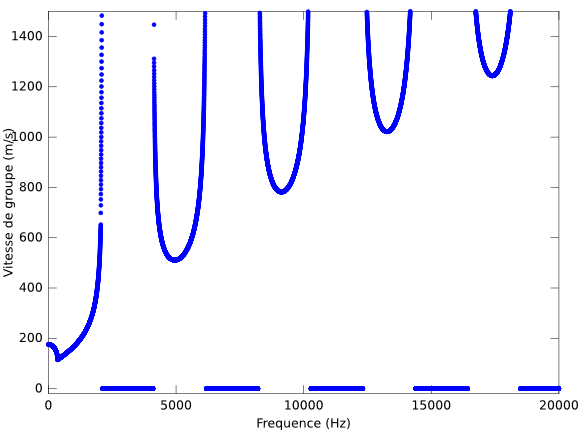
\includegraphics[width=330pt,height = 180pt]{./figures/courbe_dispersion.png}
\caption{Courbe de dispersion pour une corde lestée par des poids disposés régulièrement.}
\label{dispers}
\end{figure}

On constate que la courbe n'est pas une simple droite linéaire, le système est bien dispersif. De plus les bandes interdites sont ici clairement visibles car la vitesse de l'onde y est nulle.

\section{Impédance d'entrée}

Enfin on trace ici l'impédance d'entrée d'un système composé de $N = 33$ cellules correspondant au 33 masses utilisées dans la partie expérimentale.

La matrice de transfert de ce système est :
\begin{eqnarray*}
\begin{pmatrix} A & B \\ C & D \end{pmatrix} & = & \begin{pmatrix} T_{11} & T_{12} \\ T_{21} & T_{22} \end{pmatrix}^{N}
\end{eqnarray*}	

Par analogie avec l'électricité et en prenant une impédance de sortie infinie, l'impédance d'entrée $Z_e$ de ce système peut être calculée comme celle d'un circuit en "$\Pi$" (cf~figure~\ref{pi}).
Sur ce circuit, on a : 
\begin{equation*}
	Z_1 = \frac{D-1}{B} \text{, } \qquad Z_2 = \frac{A-1}{B} \qquad \text{et} \qquad Z_{\pi}=B
\end{equation*}

\begin{figure}[!h]
	\centering
	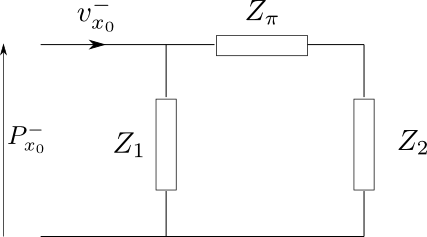
\includegraphics[scale=0.5]{./figures/schema_elec_impedance.png}
	\caption{Schéma électrique équivalent d'un réseau de N cellules.}
	\label{pi}
\end{figure}

L'expression de $Z_{e}$ est alors : 
\begin{equation*}
Z_{e} = \frac{Z_{1}(Z_{\pi}+Z_2)}{Z_1+Z_2+Z_{\pi}}
\end{equation*}
 
On obtient la courbe d'impédance présente en figure ~\ref{imp}.

\begin{figure}[!h]\centering
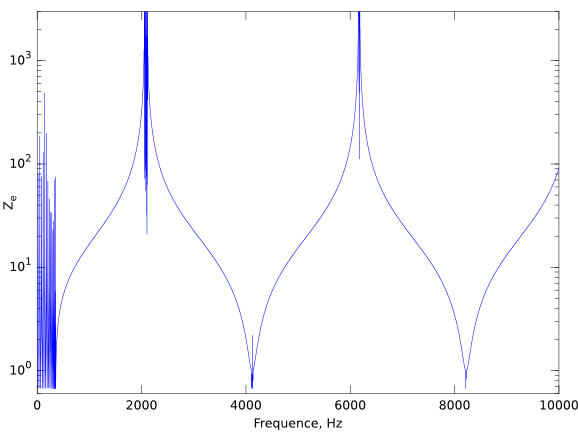
\includegraphics[width=330pt,height = 180pt]{./figures/impedance_entree.png}
\caption{Impédance d'entrée de la corde lestée pour une impédance de sortie infinie.}
\label{imp}
\end{figure}

\bigskip
Quand l'impédance est maximale, alors les ondes ne se propagent pas. On constate donc que les bandes interdites sont également visibles sur l'impédance.

Les pics présents en basses fréquences ne semble ni dus à la résonance de la corde ni à celles des masses, nous ne savons donc pas vraiment d'où viennent ces singularités.

\bigskip
Ces résultats doivent donc maintenant être confirmés par des mesures sur un banc de manipulation.
\newpage
\section{Partie expérimentale}
Le but de ce chapitre est de confirmer les différentes courbes vues au chapitre précédent.


\subsection{Protocole expérimental}
Le banc d'essai est constitué d'un fil en acier de 68~cm de masse linéique mesurée $\mu$ = 0,63~g/m sur lequel sont fixés 33 plombs de pêche de masse M=0,183~g tout les 2 cm ($=2L$). Un schéma du montage ce trouve figure ~\ref{schema_cordel}.

\begin{figure}[!h]\centering
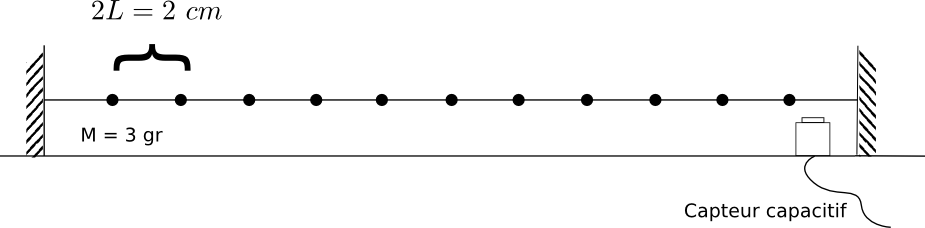
\includegraphics[scale=0.6]{./figures/schema_cordel_sans_tension.png}
\caption{Schéma du montage expérimentale.}
\label{schema_cordel}
\end{figure}

\bigskip
L'excitation est faite avec le doigt (nous n'avions pas d'excitateur magnétique et nous avons jugé le pot vibrant trop intrusif et trop compliqué à mettre en place) et l'acquisition avec un capteur capacitif placé à environ 10 cm d'une des fixations de la corde. Les données sont enregistrées via une carte d'acquisition sur le logiciel CTTM.

Seules des acquisitions de signaux temporels sont faites. Ces données sont enregistrées au format texte et audio, et sont ensuite traitées via Octave. Le signal est échantillonné à $42 000 Hz$. Étant donné que notre analyse portera en grande partie sur les basses fréquences, aucun problème lié à l'échantillonnage n'est à prévoir.
Enfin, toutes les mesures sont faites 5 fois puis moyennées.

\subsubsection{Mesure de la tension $T_0$}
On monte tout d'abord sur le banc d'essai une corde en acier sans masse à une tension suffisante (de l'ordre de celles des cordes de guitare). Une première mesure de réponse impulsionnelle est ensuite faite. On sait que la première fréquence de résonance d'une corde simple ce trouve à : $f_0 =\frac{c}{2L} = \frac{\sqrt{\frac{T_0}{\mu}}}{2L}$, comme $\mu$ est connu on peut donc en déduire $T_0$.

\bigskip
Dans un second temps, les plombs sont fixés à l'aide d'une pince sur la corde sans que celle-ci ne soit retirée afin que la tension reste la même (on estime que le poids des masses au regard de l'ordre de grandeur de la tension est négligeable). Les plombs sont placés tout les 2 centimètres.

\subsection{Résultats des mesures}
Dans un premier temps, on trace le spectrogramme de l'énergie du signal acquis dans le cas d'une corde avec 33 masses, puis sans masses. Ces résultats se trouvent en figure ~\ref{spectro}.

\begin{figure}[!h]\centering
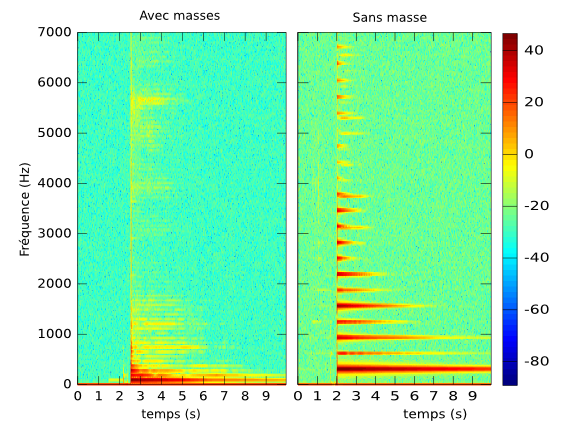
\includegraphics[scale=0.7]{./figures/spectrogram_nue.png}
\caption{Spectrogramme de l'énergie dans la corde avec et sans masses.}
\label{spectro}
\end{figure} 

Les maximums d'énergie correspondent aux résonances de la corde. Les résonances de la corde lestée sont plus rapprochées que celles de la corde sans masse du fait du changement de la masse linéique équivalente en basses fréquences.


On constate qu'une chute d'énergie est bien présente dans le cas de la corde lestée dans une bande autour de 3000~Hz et celui-ci ne se retrouve pas pour la corde seule.


\subsubsection{Causes possibles d'erreurs sur les mesures}

Cette bande interdite diffère légèrement de celle trouvée dans la partie théorique. Ceci peut être dû au calcul de la tension de la corde qui suppose que celle-ci n'a pas changé avec l'ajout des masses. De plus, la périodicité des masses a pu ne pas être parfaitement respectée du fait du placement manuel de ces dernières. Le choix des plombs de pêche est discutable car ils ne sont pas parfaitement sphériques (surtout après la pose) et certains ont tendance se déplacer légèrement après plusieurs mesures.

\bigskip
Enfin, le fait d'exciter la corde avec une simple impulsion du doigt comporte de nombreux désavantages: l'excitation de toutes les fréquences n'est pas uniforme et cela génère une onde aller et une retour dans la corde ce qui peut créer des interférences. Cependant n'ayant pas de $2^{ème}$ transducteur et jugeant que la mise en place d'un pot vibrant sur la corde serait trop intrusive, nous avons gardé la solution de l'excitation la plus simple.

\chapter*{Conclusion}
\addcontentsline{toc}{chapter}{Conclusion}

Une approche succincte de la dispersion a été faite à travers quelques exemples variés de milieux dispersifs et les différentes causes de ce phénomène ont pu être établies. 


Dans un guide d'onde, la dispersion est liée à l'impédance des parois. En effet, l'application des conditions limites pour la pression sur ces parois mène à la notion de mode, ce qui complexifie l'expression de la constante de propagation.


Dans une poutre, la prise en compte du moment de torsion fait apparaître une dérivée quatrième dans l'équation de propagation de l'onde. La résolution de cette équation conduit à une relation de dispersion.


Enfin, pour la corde lestée, la périodicité du réseau engendre la non-propagation de bande de fréquences et influe sur la célérité des ondes dont la fréquence avoisine ces bandes.
\\

Ce projet en autonomie a été mené en lien direct avec les enseignements suivis au cours de notre troisième année de licence, tels que la théorie des lignes, la propagation dans les guides d'ondes ou la mécanique.
\bigskip

\section*{Bibliographie}
\addcontentsline{toc}{section}{Bibliographie}

\indent[GUY] GUYADER, Jean-Louis. Vibrations des milieux continus. Hermes Science Publications, 2002 \\
\indent[DAL] DALMONT, Jean-Pierre. Guide des Guides d'ondes acoustiques (version 1.4). 2010 \\ 
\indent[RIC] RICHOUX, Olivier. Étude de la propagation des ondes mécaniques dans un réseau unidimensionnel comportant du désordre et/ou des non-linéarités localisées. Th. doct. : Acoustique. Le Mans : université du Maine, 1999.


%[PRON] \url{http://www.engr.uconn.edu/~sas03013/docs/PronyAnalysis.pdf}

%[COUCOU] \url{http://personnel.isae.fr/sites/personnel/IMG/pdf/slides_asp_eng.pdf}

\indent[CAS] CASTAGNEDE, Bernard. Cours de théorie des vibrations [en ligne]. Consulté le 20/05/14. Disponible à l'adresse : \\ \url{perso.univ-lemans.fr/~bcasta/Doc Enseignement/Cours M1 Vibrations(II).pdf}

\end{document}




